\chapter{Revisión de la literatura}

En este capítulo se realizará una revisión de los estudios y propuestas más innovadoras relacionadas con los algoritmos socioinspirados. Se tendrá en cuenta hasta dónde han llegado aquellos algoritmos en los que se basaron, los bioinspirados, qué impacto tienen en el panorama actual y cómo de efectivos han resultado los algoritmos socioinspirados en problemas reales hasta la fecha.

\section{Estado del arte: algoritmos bioinspirados}

La algorítmica experimentó un antes y un después con la llegada de los algoritmos bioinspirados. El planteamiento tan visual a la par que efectivo que poseen dichos algoritmos incitó que poco a poco cada vez más investigadores se dedicasen a este campo. En particular, ha tenido especial éxito en la computación evolutiva, donde las propuestas más conocidas como los algoritmos de colonias de hormigas o de colmenas de abejas han resultado no sólo innovadoras sino también efectivas.

Los algoritmos \textbf{Ant Colony Optimization (ACO)}, los basados en los comportamientos de las colonias de hormigas, han sido los pioneros en este campo. Marco Dorigo fue el padre de los ACO, publicando en su tesis doctoral \cite{dorigo-thesis} en 1992 lo que él definió como <<Ant systems>>. A partir de esta primera aproximación, Dorigo continuó su investigación en dicha técnica, y años más tarde, en 1999, publicó su primera propuesta de algoritmo, explicando, en términos del autor, lo que él propuso como <<Ant algorithms>> \cite{ant-algorithms-dorigo}.

Además de la vertiente computacional, algunas de las primeras propuestas bioinspiradas también trataban de aplicar estas técnicas al hardware, en particular a mejorar el diseño de los sistemas. Sánchez et al. (1997) plantearon la investigación en este campo. En el 1st International Conference on Evolvable Systems, acontecido en Tsukuba, Japón, en 1996, presentaron en su paper \textit{Phylogeny, ontogeny, and epigenesis: Three sources of biological inspiration for softening hardware} \cite{bioinspired-systems-paper} las bases de la investigación en técnicas bioinspiradas, en este caso para dotar a sistemas hardware de procesos evolutivos. Más adelante lo publicaron en la revista IEEE Xplore \cite{bioinspired-systems-article}.

Estos ejemplos citados no son, sin embargo, nada más que la pequeña primera muesca en la historia de las técnicas bioinspiradas. Consultando una base de datos bibliográfica se puede observar un creciente aumento en cuanto a las publicaciones relacionadas con algoritmos bioinspirados. En la base de datos de SCOPUS estos datos pueden ser plasmados en una gráfica como la que se muestra a continuación.

\begin{figure}[h]
	\centering
	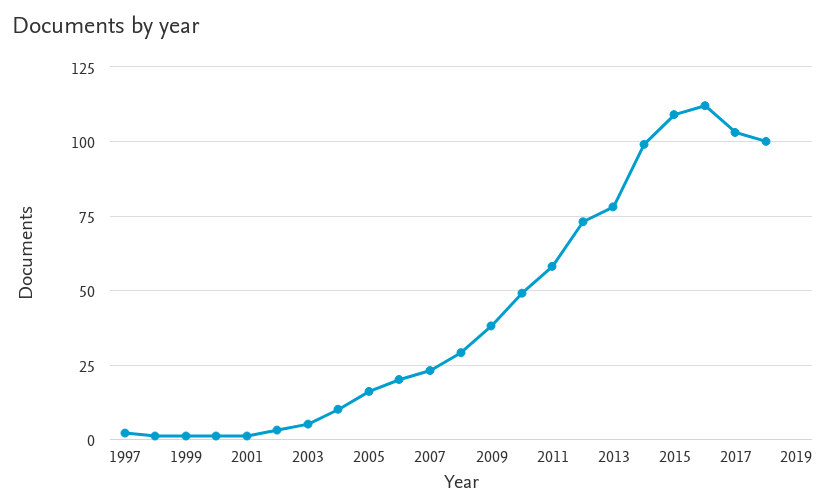
\includegraphics[scale=0.4]{imagenes/scopus-grafico-bioinspirados.png}
	\caption{Gráfico de publicaciones sobre algoritmos bioinspirados registradas en SCOPUS \cite{scopus-bioinspired}.}
\end{figure}

Dicha gráfica refleja perfectamente el auge de los algoritmos bioinspirados; de menos de diez publicaciones por año hasta el año 2004 aproximadamente, hasta los más de 100 que llevan registrándose desde 2015. El éxito de estos algoritmos se fundamenta en dos pilares: su carga conceptual es sencilla de abstraer para cualquier usuario, y generalmente aportan buenos resultados a los problemas a los que se han enfrentado.

Actualmente existen algoritmos bioinspirados en cualquier rama del reino animal. Algoritmos de manadas de lobos o grupos de tiburones que acorralan a su presa, basados en bancos de peces que se mueven en grupo hacia una zona óptima, o incluso que simulan el movimiento de una polilla cuando se dirige hacia un foco de luz. Por supuesto, con tanta diversidad no tardaron en surgir técnicas que centraban su funcionamiento en un animal muy particular: el ser humano.

\section{Estado del arte: algoritmos socioinspirados}

